\documentclass{standalone}
\usepackage{tikz}
\usetikzlibrary{patterns, positioning}

\begin{document}
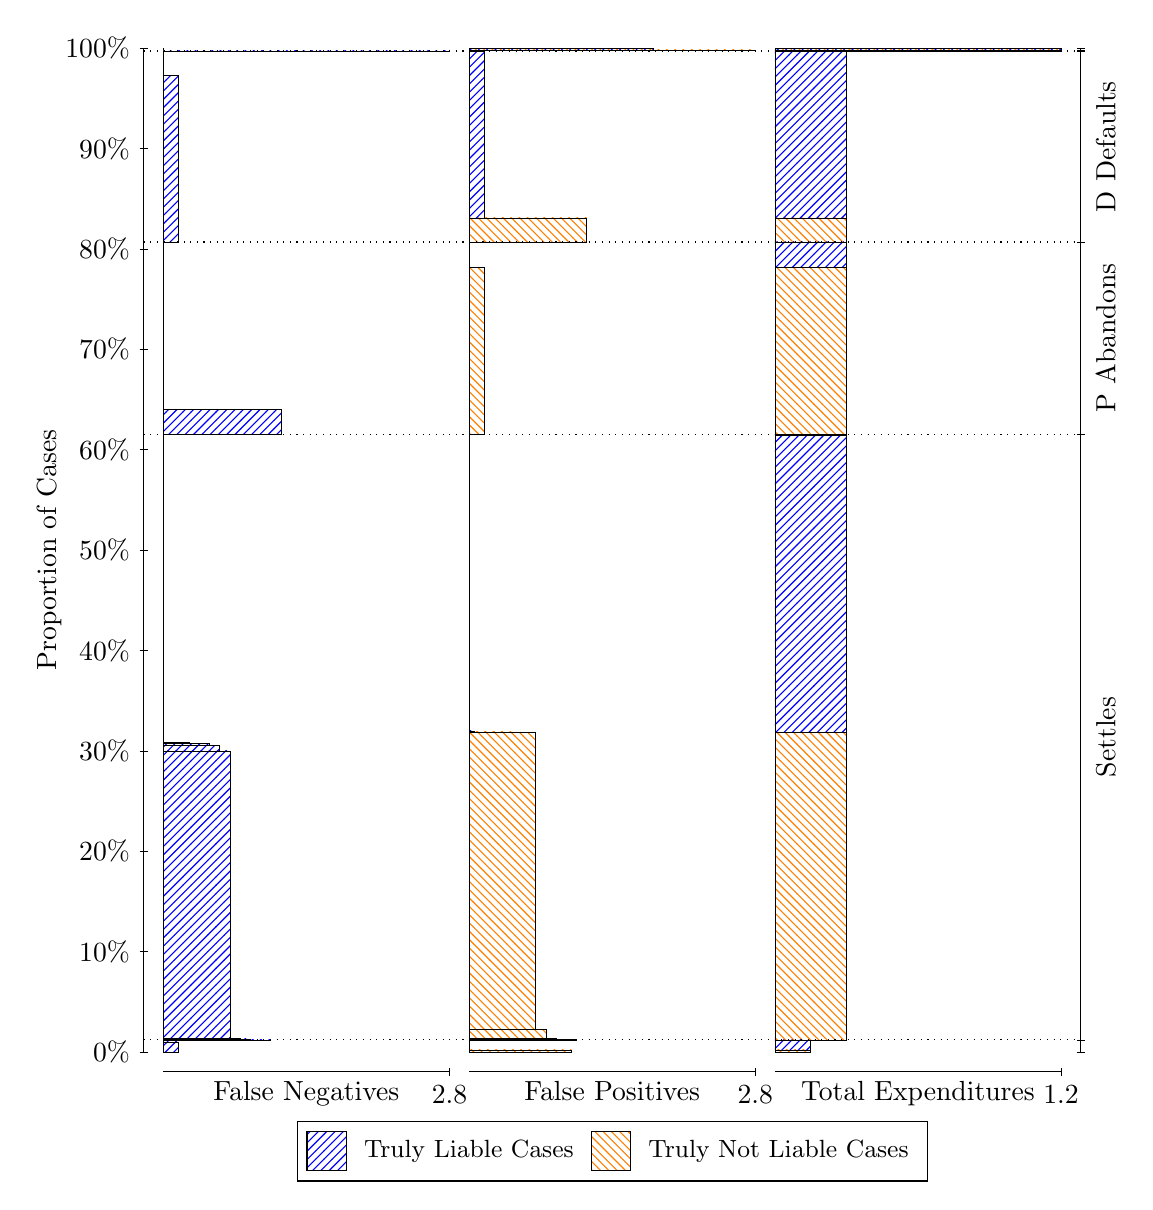
\begin{tikzpicture}
\draw[black, very thin] (1.5,1.75) -- (1.5,14.5);
\node[rotate=90, anchor=center] at (0.3, 8.125) {Proportion of Cases};
\draw[black, very thin] (1.45,1.75) -- (1.55,1.75);
\node[anchor=east] at (1.45, 1.75) {0\%};
\draw[black, very thin] (1.45,3.025) -- (1.55,3.025);
\node[anchor=east] at (1.45, 3.025) {10\%};
\draw[black, very thin] (1.45,4.3) -- (1.55,4.3);
\node[anchor=east] at (1.45, 4.3) {20\%};
\draw[black, very thin] (1.45,5.575) -- (1.55,5.575);
\node[anchor=east] at (1.45, 5.575) {30\%};
\draw[black, very thin] (1.45,6.85) -- (1.55,6.85);
\node[anchor=east] at (1.45, 6.85) {40\%};
\draw[black, very thin] (1.45,8.125) -- (1.55,8.125);
\node[anchor=east] at (1.45, 8.125) {50\%};
\draw[black, very thin] (1.45,9.4) -- (1.55,9.4);
\node[anchor=east] at (1.45, 9.4) {60\%};
\draw[black, very thin] (1.45,10.675) -- (1.55,10.675);
\node[anchor=east] at (1.45, 10.675) {70\%};
\draw[black, very thin] (1.45,11.95) -- (1.55,11.95);
\node[anchor=east] at (1.45, 11.95) {80\%};
\draw[black, very thin] (1.45,13.225) -- (1.55,13.225);
\node[anchor=east] at (1.45, 13.225) {90\%};
\draw[black, very thin] (1.45,14.5) -- (1.55,14.5);
\node[anchor=east] at (1.45, 14.5) {100\%};

\draw[black, very thin] (13.4,1.75) -- (13.4,14.5);
\draw[black, very thin] (13.35,1.75) -- (13.45,1.75);
\node[anchor=west] at (13.35, 1.75) {};
\draw[black, very thin] (13.35,1.9039) -- (13.45,1.9039);
\node[anchor=west] at (13.35, 1.9039) {};
\draw[black, very thin] (13.35,9.5971) -- (13.45,9.5971);
\node[anchor=west] at (13.35, 9.5971) {};
\draw[black, very thin] (13.35,12.037) -- (13.45,12.037);
\node[anchor=west] at (13.35, 12.037) {};
\draw[black, very thin] (13.35,14.459) -- (13.45,14.459);
\node[anchor=west] at (13.35, 14.459) {};
\draw[black, very thin] (13.35,14.471) -- (13.45,14.471);
\node[anchor=west] at (13.35, 14.471) {};
\draw[black, very thin] (13.35,14.5) -- (13.45,14.5);
\node[anchor=west] at (13.35, 14.5) {};

\draw[black, very thin, pattern color=blue, pattern=north east lines] (1.75,1.75) rectangle (1.9446,1.8774);
\draw[black, very thin, pattern color=orange, pattern=north west lines] (1.75,1.8774) rectangle (1.75,1.9039);
\draw[black, very thin, pattern color=blue, pattern=north east lines] (1.75,1.9039) rectangle (3.1125,1.9042);
\draw[black, very thin, pattern color=blue, pattern=north east lines] (1.75,1.9042) rectangle (2.9827,1.9043);
\draw[black, very thin, pattern color=blue, pattern=north east lines] (1.75,1.9043) rectangle (2.853,1.9154);
\draw[black, very thin, pattern color=blue, pattern=north east lines] (1.75,1.9154) rectangle (2.7232,1.9266);
\draw[black, very thin, pattern color=blue, pattern=north east lines] (1.75,1.9266) rectangle (2.5935,5.5752);
\draw[black, very thin, pattern color=blue, pattern=north east lines] (1.75,5.5752) rectangle (2.4637,5.6426);
\draw[black, very thin, pattern color=blue, pattern=north east lines] (1.75,5.6426) rectangle (2.3339,5.6703);
\draw[black, very thin, pattern color=blue, pattern=north east lines] (1.75,5.6703) rectangle (2.2042,5.6734);
\draw[black, very thin, pattern color=blue, pattern=north east lines] (1.75,5.6734) rectangle (2.0744,5.6866);
\draw[black, very thin, pattern color=orange, pattern=north west lines] (1.75,5.6866) rectangle (1.75,9.5971);
\draw[black, very thin, pattern color=blue, pattern=north east lines] (1.75,9.5971) rectangle (3.2423,9.9155);
\draw[black, very thin, pattern color=orange, pattern=north west lines] (1.75,9.9155) rectangle (1.75,12.037);
\draw[black, very thin, pattern color=blue, pattern=north east lines] (1.75,12.037) rectangle (1.9446,14.154);
\draw[black, very thin, pattern color=orange, pattern=north west lines] (1.75,14.154) rectangle (1.75,14.459);
\draw[black, very thin, pattern color=blue, pattern=north east lines] (1.75,14.459) rectangle (5.3833,14.464);
\draw[black, very thin, pattern color=orange, pattern=north west lines] (1.75,14.464) rectangle (1.75,14.471);
\draw[black, very thin, pattern color=orange, pattern=north west lines] (1.75,14.471) rectangle (1.75,14.476);
\draw[black, very thin, pattern color=blue, pattern=north east lines] (1.75,14.476) rectangle (1.75,14.5);
\draw[black, very thin, pattern color=orange, pattern=north west lines] (5.6333,1.75) rectangle (6.931,1.7765);
\draw[black, very thin, pattern color=blue, pattern=north east lines] (5.6333,1.7765) rectangle (5.6333,1.9039);
\draw[black, very thin, pattern color=orange, pattern=north west lines] (5.6333,1.9039) rectangle (6.9958,1.9051);
\draw[black, very thin, pattern color=orange, pattern=north west lines] (5.6333,1.9051) rectangle (6.8661,1.9057);
\draw[black, very thin, pattern color=orange, pattern=north west lines] (5.6333,1.9057) rectangle (6.7363,1.9249);
\draw[black, very thin, pattern color=orange, pattern=north west lines] (5.6333,1.9249) rectangle (6.6065,2.0381);
\draw[black, very thin, pattern color=orange, pattern=north west lines] (5.6333,2.0381) rectangle (6.4768,5.8078);
\draw[black, very thin, pattern color=orange, pattern=north west lines] (5.6333,5.8078) rectangle (6.347,5.8108);
\draw[black, very thin, pattern color=orange, pattern=north west lines] (5.6333,5.8108) rectangle (6.347,5.8109);
\draw[black, very thin, pattern color=orange, pattern=north west lines] (5.6333,5.8109) rectangle (6.2173,5.814);
\draw[black, very thin, pattern color=orange, pattern=north west lines] (5.6333,5.814) rectangle (6.0875,5.8141);
\draw[black, very thin, pattern color=orange, pattern=north west lines] (5.6333,5.8141) rectangle (5.9577,5.8144);
\draw[black, very thin, pattern color=blue, pattern=north east lines] (5.6333,5.8144) rectangle (5.6982,5.8276);
\draw[black, very thin, pattern color=blue, pattern=north east lines] (5.6333,5.8276) rectangle (5.6333,9.5971);
\draw[black, very thin, pattern color=orange, pattern=north west lines] (5.6333,9.5971) rectangle (5.828,11.718);
\draw[black, very thin, pattern color=blue, pattern=north east lines] (5.6333,11.718) rectangle (5.6333,12.037);
\draw[black, very thin, pattern color=orange, pattern=north west lines] (5.6333,12.037) rectangle (7.1256,12.342);
\draw[black, very thin, pattern color=blue, pattern=north east lines] (5.6333,12.342) rectangle (5.828,14.459);
\draw[black, very thin, pattern color=orange, pattern=north west lines] (5.6333,14.459) rectangle (5.6333,14.466);
\draw[black, very thin, pattern color=blue, pattern=north east lines] (5.6333,14.466) rectangle (5.6333,14.471);
\draw[black, very thin, pattern color=orange, pattern=north west lines] (5.6333,14.471) rectangle (9.2667,14.476);
\draw[black, very thin, pattern color=blue, pattern=north east lines] (5.6333,14.476) rectangle (7.969,14.5);
\draw[black, very thin, pattern color=orange, pattern=north west lines] (9.5167,1.75) rectangle (9.9708,1.7765);
\draw[black, very thin, pattern color=blue, pattern=north east lines] (9.5167,1.7765) rectangle (9.9708,1.9039);
\draw[black, very thin, pattern color=orange, pattern=north west lines] (9.5167,1.9039) rectangle (10.425,5.8108);
\draw[black, very thin, pattern color=blue, pattern=north east lines] (9.5167,5.8108) rectangle (10.425,9.5819);
\draw[black, very thin, pattern color=orange, pattern=north west lines] (9.5167,9.5819) rectangle (10.425,9.5823);
\draw[black, very thin, pattern color=blue, pattern=north east lines] (9.5167,9.5823) rectangle (10.425,9.5825);
\draw[black, very thin, pattern color=orange, pattern=north west lines] (9.5167,9.5825) rectangle (10.425,9.5857);
\draw[black, very thin, pattern color=blue, pattern=north east lines] (9.5167,9.5857) rectangle (10.425,9.5971);
\draw[black, very thin, pattern color=orange, pattern=north west lines] (9.5167,9.5971) rectangle (10.425,11.718);
\draw[black, very thin, pattern color=blue, pattern=north east lines] (9.5167,11.718) rectangle (10.425,12.037);
\draw[black, very thin, pattern color=orange, pattern=north west lines] (9.5167,12.037) rectangle (10.425,12.342);
\draw[black, very thin, pattern color=blue, pattern=north east lines] (9.5167,12.342) rectangle (10.425,14.459);
\draw[black, very thin, pattern color=orange, pattern=north west lines] (9.5167,14.459) rectangle (13.15,14.466);
\draw[black, very thin, pattern color=blue, pattern=north east lines] (9.5167,14.466) rectangle (13.15,14.471);
\draw[black, very thin, pattern color=orange, pattern=north west lines] (9.5167,14.471) rectangle (13.15,14.476);
\draw[black, very thin, pattern color=blue, pattern=north east lines] (9.5167,14.476) rectangle (13.15,14.5);
\draw[black, dotted] (1.5,1.9039) -- (13.4,1.9039);
\draw[black, dotted] (1.5,9.5971) -- (13.4,9.5971);
\draw[black, dotted] (1.5,12.037) -- (13.4,12.037);
\draw[black, dotted] (1.5,14.459) -- (13.4,14.459);
\draw[black, dotted] (1.5,14.471) -- (13.4,14.471);
\draw[black, very thin] (1.75,1.5) -- (5.3833,1.5);
\node[anchor=north] at (3.5667, 1.5) {False Negatives};
\draw[black, very thin] (5.3833,1.45) -- (5.3833,1.55);
\node[anchor=north] at (5.3833, 1.45) {2.8};

\draw[black, very thin] (5.6333,1.5) -- (9.2667,1.5);
\node[anchor=north] at (7.45, 1.5) {False Positives};
\draw[black, very thin] (9.2667,1.45) -- (9.2667,1.55);
\node[anchor=north] at (9.2667, 1.45) {2.8};

\draw[black, very thin] (9.5167,1.5) -- (13.15,1.5);
\node[anchor=north] at (11.333, 1.5) {Total Expenditures};
\draw[black, very thin] (13.15,1.45) -- (13.15,1.55);
\node[anchor=north] at (13.15, 1.45) {1.2};


\node[black, centered, rotate=90] at (13.72, 5.7505) {Settles};
\node[black, centered, rotate=90] at (13.72, 10.817) {P Abandons};
\node[black, centered, rotate=90] at (13.72, 13.248) {D Defaults};



\draw (7.449999999999999,1.5) node[draw=none] (baseCoordinate) {};
\begin{scope}[align=center]
        \matrix[scale=0.5, draw=black, below=0.5cm of baseCoordinate, nodes={draw}, column sep=0.1cm]{
            \node[rectangle, draw, minimum width=0.5cm, minimum height=0.5cm, pattern=north east lines, pattern color=blue] {}; &
            \node[draw=none, font=\small] (B) {Truly Liable Cases}; &
            \node[rectangle, draw, minimum width=0.5cm, minimum height=0.5cm, pattern=north west lines, pattern color=orange] {}; &
            \node[draw=none, font=\small] (B) {Truly Not Liable Cases}; \\
            };
\end{scope}

\end{tikzpicture}
\end{document}